\section{Гармонические функции в $\R^3$ и их свойства. Бесконечная дифференцируемость гармонических функций. Теорема о среднем. Обратная теорема о среднем. Теоремы Лиувилля и об устранимой особой точке (случай $\R^3$).}
% Затехала Ермолова Марина
\begin{definition} Функция $u(x)$ гармоническая в $\Omega \in \R^3$, если 
\begin{enumerate}
\item $u(x) \in C^2 (\Omega)$
\item $\Delta u(x) = 0 \Forall x \in \Omega$ 
\end{enumerate}
\end{definition}
\begin{theorem}
Всякая функция $u(x)$, гармоническая в области $\Omega$, является в $\Omega$ бесконечно дифференцируемой, т.е. $u(x) \in C^{\infty}(\Omega).$
\end{theorem}
\begin{proof}
Возьмем $x_0 \in \Omega$ и $\overline{B_r(x_0)} \subset \Omega$. Представим $u(x)$ суммой: $$u(x)= - \oint\limits_{|y-x_0|=r} \bigg( -\frac{1}{4\pi |x-y|} \bigg) \frac{\partial u(y)}{\partial {n_y}} dS_y + \oint\limits_{|y-x_0|=r} u(y) \frac{\partial}{\partial \vec{n}_y} \bigg(-\frac{1}{4\pi |x-y|}\bigg) dS_y $$
\begin{center}
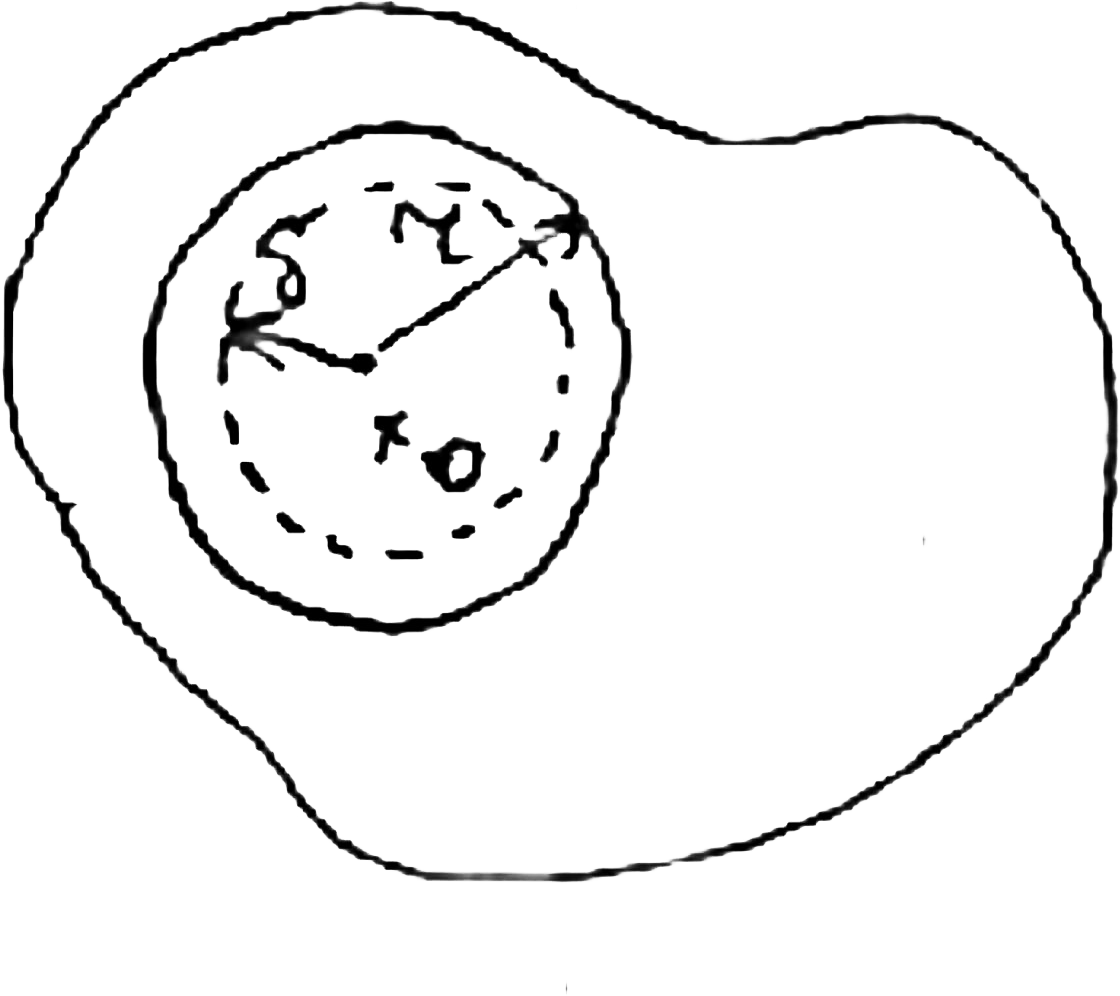
\includegraphics[width=0.2\textwidth]{21_1_new}
\end{center}
Теперь берем $B_{\delta}(x_0) \subsetneq B_{r}(x_0).$ Будем обозначать $S(x_0,r)$ сферу $\partial B_r(x_0).$ Если $x \in \overline{B_{\delta}(x_0)}, y \in S(x_0,r)$, то $|x-y| \geq r - \delta > 0.$\\
Рассмотрим в $\overline{B_{\delta}(x_0)}$ $$u_0(x)= \oint\limits_{|y-x_0|=r} \bigg( -\frac{1}{4\pi |x-y|} \bigg) \frac{\partial u(y)}{\partial \vec{n}_y} dS_y.$$
Напишем $$\tilde{u}_0(x) = \oint\limits_{|y-x_0|=r} D_x^\alpha \bigg( -\frac{1}{4\pi |x-y|} \bigg) \frac{\partial u(y)}{\partial \vec{n}_y} dS_y$$
Заметим, что $-\frac{1}{4\pi |x-y|} \in C^{\infty}( \overline{B_{\delta}(x_0)} \times S(x_0,r)) \Rightarrow$ записанные частные производные непрерывны, интеграл $\tilde{u}_0$ существует $\Rightarrow \tilde{u}_0(x) = D_x^\alpha u_0(x).$\\
Теперь берем $$u_2(x) = \oint\limits_{|y-x_0|=r} u(y) \frac{\partial}{\partial \vec{n}_y} \bigg(-\frac{1}{4\pi |x-y|}\bigg) dS_y$$ 
$$\frac{\partial}{\partial \vec{n}_y} \bigg(-\frac{1}{4\pi |x-y|}\bigg) = \sum_{k=1}^n n_k \frac{\partial}{\partial y_k} \bigg(-\frac{1}{4\pi |x-y|}\bigg)$$ В $\overline{B_{\delta}(x_0)}$ запишем 
$$\tilde{u}_2(x)=\sum_{k=1}^3 \oint\limits_{|y-x_0|=r} u_(y) n_k (y) D_x^\alpha \bigg(\frac{\partial}{\partial y_k} \bigg(-\frac{1}{4\pi |x-y|}\bigg)\bigg)dS_y$$
Записанные частные производные непрерывны, интеграл $\tilde{u}_2(x)$ существует $\Rightarrow \tilde{u}_2(x)=D_x^\alpha u_2(x).$\\
Итак, для $u_0(x)$ и $u_2(x)$ существуют частные производные любого порядка. Значит, $u(x) \in  C^{\infty}( \overline{B_{\delta}(x_0)}),$ где\\ $x_0$ -- произвольная точка из $\Omega \Rightarrow u(x) \in C^{\infty}(\Omega)$
\end{proof}
\begin{theorem}[Теорема о среднем]
Пусть $u(x)$, гармоническая в шаре $B_r(x_0)$ и $u(x) \in C^1(\overline{B_r(x_0)})$. Тогда $$u(x_0)= \frac{1}{4\pi r^2} \int \limits_{|y-x_0|=r}u(y)dS_y$$ (в центре -- среднее по значениям на сфере)
\end{theorem}
\begin{proof}
$$u(x_0)= -\oint\limits_{|y-x_0|=r} \bigg( -\frac{1}{4\pi |x_0-y|} \bigg) \frac{\partial u}{\partial \vec{n}_y} dS_y + \oint\limits_{|y-x_0|=r} u(y) \frac{\partial}{\partial \vec{n}_y} \bigg(-\frac{1}{4\pi |x_0-y|}\bigg) dS_y $$
$$\frac{\partial}{\partial \vec{n}_y} \bigg(-\frac{1}{4\pi |x_0-y|}\bigg)\stackrel{\rho = |x_0 - y|}{=} -\frac{1}{4\pi}\frac{\partial}{\partial \rho}\frac{1}{\rho} = \frac{1}{4 \pi r^2},$$ тогда $$\oint\limits_{|y-x_0|=r} u(y) \frac{\partial}{\partial \vec{n}_y} \bigg(-\frac{1}{4\pi |x_0-y|}\bigg) dS_y = \frac{1}{4 \pi r^2} \oint\limits_{|y-x_0|=r} u(y) dS_y.$$
Покажем, что потенциал простого слоя равен нулю.
\[ -\oint\limits_{|y-x_0|=r} \bigg( -\frac{1}{4\pi |x_0-y|} \bigg) \frac{\partial u(y)}{\partial \vec{n}_y} dS_y = \frac{1}{4\pi} \frac{1}{r} \oint\limits_{|y-x_0|=r}  \frac{\partial u(y)}{\partial \vec{n}_y} dS_y = \frac{1}{4\pi r} \oint\limits_{|y-x_0|=r} (\nabla u(y), \vec{n}(y)) dS_y \stackrel{\text{ф-ла Остр.--Гаусса}}{=}
\]
\[
 = \frac{1}{4\pi r} \oint\limits_{|y-x_0|<r} \div(\nabla u) dy = \frac{1}{4\pi r} \oint\limits_{|y-x_0|<r} \Delta u dy  = 0
 \]
\end{proof}
\begin{theorem}[Обратная теорема о среднем]
Пусть $u(x) \in C(\Omega)$ и $u(x)$ обладает свойством среднего $\forall x \in \Omega$, где $\Omega \in \R^3$ -- произвольная область. Тогда $u(x)$ -- гармоническая функция на $\Omega$. 
\end{theorem}
\begin{proof}
$\forall x_0\in\Omega\Exists R > 0: \overline{B(x_0, R)}\subset\Omega.$ 
Рассмотрим решение $$v(x) = \frac{1}{4\pi R}\oint\limits_{|y|=R}\frac{R^2-|x|^2}{|y-x|^3}u(y)dS_y $$ 
$$\text{для задачи} \begin{cases}
\Delta v(x) = 0, |x| < R \\
\eval{v}_{|x| = R} = \eval{u}_{|x| = R}
\end{cases} $$
Введем $w(x) = u(x) - v(x)$, $w(x) \in C(|x| \leq R)$, получим что $w(x)$ удовлетворяет свойству среднего. Тогда по принципу максимума (для функции, удовлетворяющей свойству среднего, будет доказан в следующем билете) $|w(x)| \leq \max\limits_{|y-x| = R}|w(y)| = 0  \Rightarrow u(x) = v(x) \Forall x\colon |x| < R$.
\end{proof}



% Затехал: Дмитрий Федоряка
\Subsection{Теорема Лиувилля}

\begin{theorem}

{\bf (Теорема Лиувилля)} Функция $u(x)$, гармоническая в $\R^3$ ($\Delta u = 0$)  и имеющая на бесконечности рост не выше степенного (т.е. $|u(x)| \le C (1+|x|)^{\mu}$), является многочленом от $x_1,x_2,x_3$ степени не выше $\mu$.

\end{theorem}

\Subsection{Доказательство при $\mu \ge 0$}

Общая идея -- доказать, что все производные степени выше $\mu$ равны нулю.


\begin{enumerate}



\item{

Выберем $x \in \R^3, R>0$ так, чтобы $R > 2|x|$:
\begin{center}
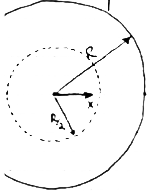
\includegraphics{21_2_new}
\end{center}
В области $|x|<R$ $u(x)$ -- гармоническая, а $\left. u(x) \right|_{\partial \Omega} \in C(\partial \Omega)$.

Тогда применима формула Пуассона для шара:

$$u(x) = \frac{1}{4 \pi R} \oint_{|y|=R}{\frac{R^2-|x|^2}{|y-x|^3} u(y) dS_y }
$$

В силу выбора $R$ имеем $|y-x| \ge |y|- |x| \ge \frac{R}{2} >0$.

Можем записать:

$$D_{x}^{\alpha} u(x) = \frac{1}{4 \pi R} 
\oint_{|y|=R}{D_{x}^{\alpha}\brk*{\frac{R^2-|x|^2}{|y-x|^3}}u(y) dS_y}$$

}





\item{

Докажем по индукции, что
 
$$\forall \alpha = (\alpha_1,\alpha_2,\alpha_3)~~~ D_{x}^{\alpha}\brk[s]*{\frac{R^2-|x|^2}{|x-y|^3}} = \frac{P_{\alpha}(R,x,y)}{|x-y|^{3+2|\alpha|}},$$

где $P_\alpha$ -- однородный многочлен степени $|a|+2$ от $R, x_1,x_2,x_3,y_1,y_2,y_3$.


\begin{itemize}
	\item {База:}
	
	$$D_{x}^{(0,0,0)}\brk[s]*{\frac{R^2-|x|^2}{|x-y|^3}} = \frac{R^2-x_1^2-x_2^2-x_3^2}{|x-y|^3}$$
	
	\item {Переход. 
Пусть требуемое верно $\forall \alpha: |a|\le k$. Возьмём $\hat{\alpha}=(\alpha_1+1, \alpha_2, \alpha_3)$:}

$$
D_{x}^{\hat{\alpha}}\brk[s]*{\frac{R^2-|x|^2}{|x-y|^3}} = \frac{\partial}{\partial x_1}
\brk[s]*{\frac{P_{\alpha}(R,x,y)}{|x-y|^{3+2|\alpha|}}}
=
\frac{
\frac{\partial P_{\alpha}}{\partial x_1} \cdot |x-y|^2 - (3+2|\alpha|)\cdot P_\alpha \cdot (x_1-y_1)
}
{|x-y|^{3+2(|\alpha|+1)}}
=
\frac{P_{\hat{\alpha}}(R,x,y)}{|x-y|^{3+2|\hat{\alpha}|}}
$$ 
	
\end{itemize}
}



\item{
Покажем теперь, что $\forall |x| \le \frac{R}{2}, \Forall |y|=R, \Forall \alpha =(\alpha_1,\alpha_2,\alpha_3)$ справедлива оценка:

$$\left| D_{x}^{\alpha}\brk*{\frac{R^2-|x|^2}{|x-y|^3}} \right| \le \frac{C_\alpha}{R^{1+|\alpha|}}.
$$

Действительно, $|P_\alpha| \le \tilde{C}_\alpha R^{|a|+2}$, а $|x-y|^{3+2|\alpha|} \ge \brk*{\frac{R}{2}}^{3+2|\alpha|} = \hat{C_\alpha}R^{3+2|\alpha|}$. Отсюда следует требуемая оценка.
}

\item{

Теперь докажем, что $D_x^\alpha u(x) = 0 \Forall \alpha\colon |\alpha|>\mu$.

$$
\left| D_x^{\alpha} u(x) \right| = \frac{1}{4 \pi R} 
\left|
\oint_{|y|=R}{D_x^{\alpha}\brk*{\frac{R^2-|x|^2}{|y-x|^3}}u(y)dS_y}
\right|
\le
\frac{1}{4 \pi R} \cdot C \cdot (1+ |x|)^\mu \cdot 
\frac{C_\alpha}{R^{1+|a|}} \cdot 4 \pi R^2 
\le$$ 
$$
\le
\frac{C \cdot C_\alpha \cdot (1+R)^\mu}{R^{|\alpha|}} 
\underset{R \to \infty}{\longrightarrow}
0. ~~
\text{Значит,}~~ D_x^{\alpha} u(x)=0 \Forall x \in \R^3, |\alpha|>\mu .$$

} 


\item{

Для гармонической в $\R^3$ функции $u(x)$ справедливо представление:

$$
u(x) = u(0) + \sum_{k=1}^{m} \sum_{|\alpha|=k} \frac{1}
{\alpha_1! \alpha_2! \alpha_3!} D_x^{\alpha} u(0) 
x_1^{\alpha_1}x_2^{\alpha_2}x_3^{\alpha_3}
+
\sum_{k=m+1}^{\infty} \sum_{|\alpha|=k} \frac{1}
{\alpha_1! \alpha_2! \alpha_3!} \underset{=0}{D_x^{\alpha} u(0)}
x_1^{\alpha_1}x_2^{\alpha_2}x_3^{\alpha_3}
=
$$

$$
=
u(0) + \sum_{k=1}^{m} \sum_{|\alpha|=k} \frac{1}
{\alpha !} D_x^{\alpha} u(0) 
x^{\alpha},
$$

где $m = [\mu], \, \alpha ! \triangleq \alpha_1!\alpha_2!\alpha_3!, \, x^\alpha \triangleq x_1^{\alpha_1}x_2^{\alpha_2}x_3^{\alpha_3}$.



}

\end{enumerate}






\Subsection{Доказательство при $\mu < 0$}

Пусть $\mu<0$. Тогда т.к. $|u(x)|\le C(1+|x|)^\mu, \mu<0$, то
$|u(x)| \le C (1+|x|)^0 \equiv C_1$. 

По предыдущему пункту, $u(x)$ -- полином степени 0, т.е. константа.

Но $|u(x)| \le \frac{C}{(1+|x|)^{|\mu|}} \Rightarrow u(x) 
\underset{|x| \to \infty}{\longrightarrow}
0   \Rightarrow u(x) \equiv 0$.



% Затехал: Дмитрий Федоряка
\Subsection{Теорема об устранимой особой точке}

\begin{theorem}

{\bf (об  устранимой особой точке).} 
Пусть $u(x)$ -- гармоническая в $\mathring{B}_\rho(a) \subset 
\R^3$ и $u(x)=o(E(x-a))$ при $x \to a$, где $E(x) = -\frac{1}{4 \pi |x|}$. Тогда $u(x)$ можно так доопределить в точке $a$, что она будет гармонической в $B_\rho(a) = \{x: |x-a|<\rho \}$.

\end{theorem}

\textbf{Доказательство.}


\begin{enumerate}
\item{ 
	
	$u(x) = o \brk*{\frac{1}{|x|}} \Leftrightarrow |x| \cdot u(x) 
	\underset{x \to 0}{\longrightarrow} 0$
}

\item{
Возьмём $r<\rho$. 
\begin{center}
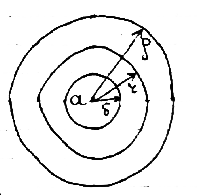
\includegraphics{21_3_new}
\end{center}
Функция $u(x)$ непрерывна на $\partial B_r (a)$.

Построим гармоническую функцию:

$$\hat{u}(x) = \frac{1}{4 \pi r} 
\oint_{|y|=r}\frac{r^2 - |x|^2}{|y-x|^3} u(y) dS_y \in 
C(|x| \le r)$$.

}


\item{

Считаем $a=0$. Покажем, что $u(x) \equiv \hat{u}(x)$ при $0<|x|\le r$. Строим $v(x) = u(x) - \hat{u}(x)$. Эта функция гармоническая в $\mathring{B}_r(a)$, непрерывная на $(0<|x| \le r)$, а также 
$v(x) \equiv 0 \Forall x: |x|=r$ и $|x| \cdot v(x) \underset{x \to 0}{\longrightarrow} 0$. 
 
}

\item{

Фиксируем $\varepsilon >0$ и рассмотрим функции $W_\eps^{\pm} =
\frac{\varepsilon}{|x|} \mp v(x)$.

Функции $W_\eps^{\pm}$ также гармонические в $(0<|x|<r)$, непрерывны на $(0<|x| \le r)$, а 
$\left.W_\eps^{\pm}(x) \right|_{|x|=r} =\frac{\eps}{|x|} >0$.
}

\item{

Выберем $\delta > 0 $ так, чтобы $\forall x:~~ |x| \le \delta \to |x| \cdot |v(x)| < \frac{\varepsilon}{2}$.

При $|x|\le \delta$: 

$$
W_\varepsilon^{\pm} = \frac{\eps}{|x|} \mp v(x) \ge 
\frac{\eps}{|x|} - |v(x)|
\ge 
\frac{\eps}{|x|}\brk[s]*{1 - \frac{|x|\cdot |v(x)|}{\varepsilon}}
\ge
\frac{\eps}{|x|}\brk[s]*{1-\frac{1}{2}}
=
\frac{\varepsilon}{2|x|} >0
$$
}



\item{

При $\delta \le |x| \le r$  функции $W_\eps^{\pm}(x)$
 -- гармонические в $(\delta < |x| < r)$ и непрерывны на замыкании 
этой ограниченной области $\Rightarrow$ по принципу максимума 
максимум и минимум достигаются на границе.

Значит, $W_\varepsilon^{\pm} (x) > 0$ при $\delta \le |x| \le r$.

Итак, $W_\varepsilon^\pm(x)$ положительна в $(0<|x| \le r)$
$\Rightarrow$  $|v(x)| < \frac{\varepsilon}{|x|}$ в $(0<|x|\le r)$.

Значит, $v(x) \equiv 0$ при $0<|x|\le r$ $\Rightarrow$ $v(x)$ можно продолжить на $|x|\le r$, положив $v(0)=0$, ч.т.д. 

}

\end{enumerate}
